% Created 2022-10-25 mar 21:02
% Intended LaTeX compiler: pdflatex
\documentclass[12pt]{article}
\usepackage[utf8]{inputenc}
\usepackage[T1]{fontenc}
\usepackage{graphicx}
\usepackage{grffile}
\usepackage{longtable}
\usepackage{wrapfig}
\usepackage{rotating}
\usepackage[normalem]{ulem}
\usepackage{amsmath}
\usepackage{textcomp}
\usepackage{amssymb}
\usepackage{capt-of}
\usepackage{hyperref}
\usepackage[spanish]{babel}
\usepackage{graphicx,geometry}
\geometry{ a4paper, left=1in, right=1in, top=1in, bottom=1in }
\renewcommand\familydefault{\sfdefault}
\usepackage{sectsty}
\sectionfont{\normalfont\Large }
\subsectionfont{\normalfont}
\usepackage{tabularx}
\usepackage{listings}
\lstdefinestyle{mystyle}{
numbers=left,
showspaces=false,
frame=leftline,
showspaces=false,
showstringspaces=false,
showtabs=false,
numberstyle=\tiny,
}
\lstset{
style=mystyle,
literate={á}{{\'a}}1
{é}{{\'e}}1
{í}{{\'{\i}}}1
{ó}{{\'o}}1
{ú}{{\'u}}1
{Á}{{\'A}}1
{É}{{\'E}}1
{Í}{{\'I}}1
{Ó}{{\'O}}1
{Ú}{{\'U}}1
{ü}{{\"u}}1
{Ü}{{\"U}}1
{ñ}{{\~n}}1
{Ñ}{{\~N}}1
{¿}{{?``}}1
{¡}{{!``}}1
}
\makeatletter
\usepackage{fancyhdr}
\pagestyle{fancy}
\usepackage{mdframed}
\BeforeBeginEnvironment{minted}{\begin{mdframed}}
\AfterEndEnvironment{minted}{\end{mdframed}}
\author{Luis Eduardo Galindo Amaya (1274895)}
\date{21-10-2022}
\title{Instrucciones de control de flujo.}
\hypersetup{
 pdfauthor={Luis Eduardo Galindo Amaya (1274895)},
 pdftitle={Instrucciones de control de flujo.},
 pdfkeywords={},
 pdfsubject={},
 pdfcreator={Emacs 26.3 (Org mode 9.1.9)}, 
 pdflang={Spanish}}
\begin{document}



\newcommand{\docente}{Arturo Arreola Alvarez}
\newcommand{\asignatura}{Organización de Computadoras (331)}
\newcommand{\semestre}{2022-2}

\newcommand{\miportada}[1]{
	\begin{titlepage}
		\vspace*{0.75in}
		\begin{flushleft}
			\sffamily
			\large #1       \\
			\Huge 
            \@title         \\
			\hrulefill
			\vspace{0.25in} \\
			\Large \@author \\
			\vspace*{\fill}
            
\includegraphics[width=\textwidth]{../includes/filler.png} \\
			\vspace*{\fill}
			\large
			\begin{tabular}{|l|l|}
              \hline
			  Asignatura & \asignatura \\
			  Docente    & \docente    \\
			  Fecha      & \@date      \\
              \hline
			\end{tabular}
		\end{flushleft}
	\end{titlepage}
}

\miportada{ Práctica 9 }

\fancyhf{}
\lhead{ \asignatura }
\rhead{ \semestre }
\rfoot{Página \thepage}

\setlength\parindent{0pt}   % eliminar el intentado
\setlength{\parskip}{1.2em}
\maketitle

\section*{Objetivo}
\label{sec:org31b68e0}
Seleccionar las instrucciones de control de flujo del programa adecuadas, para
desarrollar aplicaciones de sistemas basados en microp

\section*{Desarrollo}
\label{sec:orgca0430b}
Programe las siguientes rutinas usando las instrucciones de control de flujo del
procesador 80386 y las rutinas en la biblioteca de funciones libpc\_io.a. Escriba su
código fuente en un archivo llamado P8.asm, ensamble el código con NASM y
encadénelo con el comando ld.

\subsection*{a) gets}
\label{sec:org19494f9}
Almacena en memoria una cadena de caracteres ingresada por el usuario por medio
del teclado. La captura termina cuando el usuario presiona la tecla ENTER. La 
cadena se almacena a partir de la dirección EDX y con un 0 (null) al final que 
indica el fin de cadena. Cuando el usuario teclea la cadena, se deben 
visualizar en pantalla los caracteres ingresados.

Una vez que tenga funcional la rutina, modifíquela de forma que acepte la tecla
BACKSPACE. Cada que el usuario presiona esta tecla, el último carácter de la 
cadena es borrado de pantalla y de memoria. La rutina no debe usar gotoxy, 
haga uso de getch/getche y putchar.

\textbf{Información}: El código ASCII de la tecla ENTER es 10. El BACKSPACE es 8. Se 
hace uso de getch/getche para recibir cada carácter individual del teclado y 
se verifica si se recibió un ENTER ó BACKSPACE, para proceder a terminar la 
captura o hacer el borrado del último carácter ingresado.

\subsection*{b) getsAlpha}
\label{sec:orge34ba3d}
El procedimiento es similar a gets, a excepción de que sólo acepta caracteres
del abecedario a – z y A – Z.

\subsection*{c) asteriscos}
\label{sec:org595665a}
Colocar en CX la cantidad de renglones con asteriscos se desean imprimir. El
procedimiento imprime las líneas con asteriscos. La primera línea cuenta con 
1 asterisco, la segunda con 2, etc. Ejemplo: Si CX = 5 el procedimiento debe 
imprimir:

\begin{verbatim}
*
**
***
****
*****
\end{verbatim}




\section*{Capturas}
\label{sec:orga2968c0}
\begin{figure}[htbp]
\centering
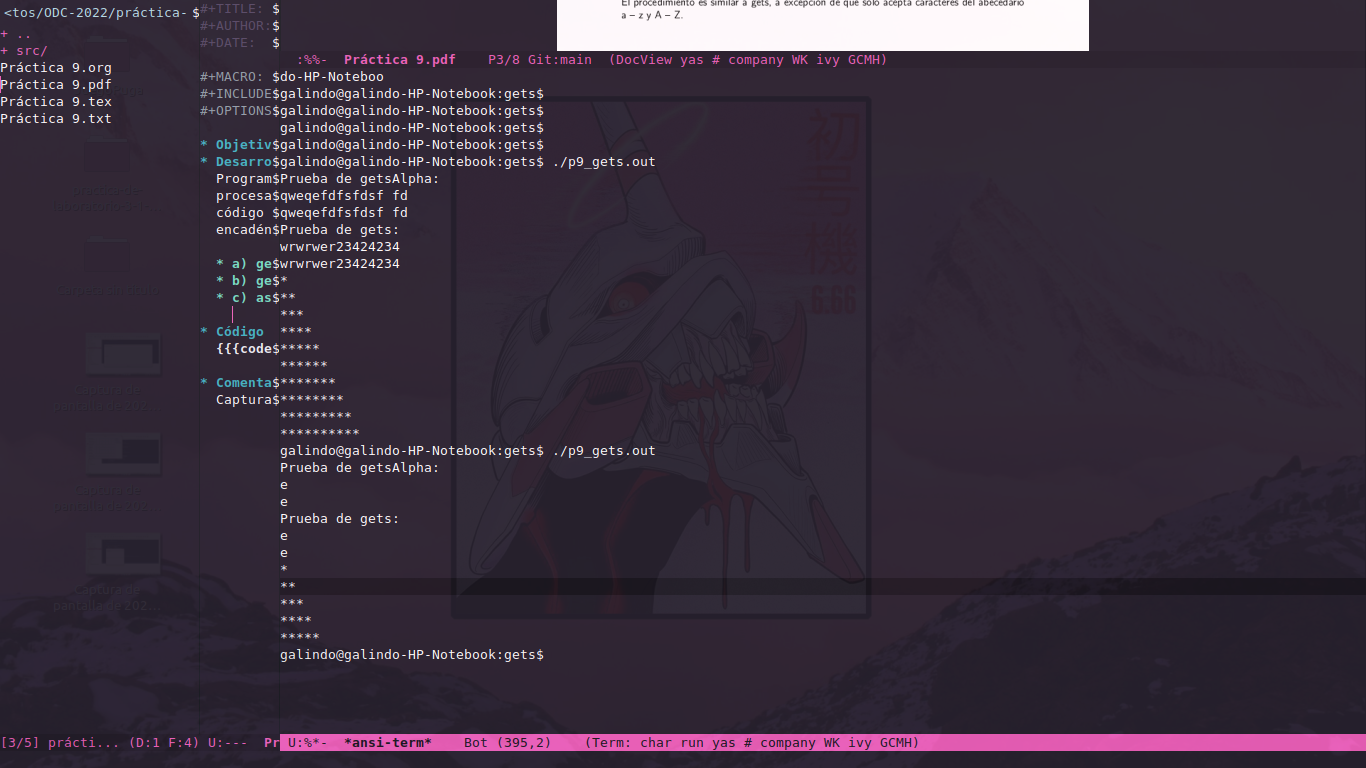
\includegraphics[width=10cm]{img/1.png}
\caption{Programa funcionando}
\end{figure}

\section*{Código}
\label{sec:orgf3426a7}
\\ \lstinputlisting{./src/P9.asm}

\section*{Comentarios}
\label{sec:org185f25b}
Capturar cosas con asembly no es facil, pero es un desafio interesante.
\end{document}
